\documentclass[./main.tex]{subfiles}



\begin{document}
\chapter{Il Theorem prover Vampire} \label{chap:vampire}
\textit{Vampire} \cite{vampire1} \cite{vampire2} \cite{vampireWebsite} è un dimostratore di teoremi automatico
per la logica del primo ordine basato sulle regole di \textit{Resolution} e \textit{Paramodulation}.
Nasce nel 1998 come progetto di ricerca degli autori Andrei Voronkov e Alexandre Riazanov,
adesso è correntemente mantenuto e sviluppato da un team più ampio presso il dipartimento di Computer Science dell'Università di Manchester. 
Il software è open-source, sviluppato in C++ e al momento della scrittura di questa tesi è giunto alla versione 4.8 con licenza BSD-3.
Vampire incorpora un complesso sistema strutture dati, algoritmi per la manipolazione di formule e termini e un vasto sistema di inferenze.
Uno dei suoi punti di forza è l'efficienza, Il team di sviluppo infatti partecipa annualmente al \textit{CASC} (The CADE ATP System Competition),
una competizione tra sistemi ATP, e fino ad ora ha sempre vinto almeno in una categoria ogni anno.
Questa ambizione per l'efficienza ha influenzato molto la struttura di Vampire e la sua implementazione.
Questo è sia un lato positivo che negativo, infatti se da un lato ci si ritrova con funzioni efficienti e ben ottimizzate,
dall'altro lato ci si ritrova spesso con un codice complesso e difficile da comprendere che predilige la velocità alla pulizia.
Ogni suo componente è riconducibile ad un articolo che ne spiega il funzionamento ad alto livello ma spesso
alcune scelte implementative sono poco o per nulla documentate. 
Spesso lo stesso nome di una funzione o di una classe fa intuire il suo scopo e funzionamento ma 
non sempre è così e altrettanto spesso si è costretti a fare 'Reverse Engineering' del codice sorgente per capire come è stato utilizzato in altri contesti.
Questo è un problema di cui il team di sviluppo è consapevole e negli ultimi anni sta cercando di migliorare.
\begin{figure}[ht]
    \centering
    \includesvg{images/3_vampire/vampire_cartelle.svg}
    \caption{Struttura delle cartelle di Vampire.}
    \label{fig:vampire_cartelle}
\end{figure}
In questo capitolo si cercherà di dare una panoramica generale di Vampire, spiegando le sue componenti principali e come queste interagiscono tra di loro,
con un focus particolare su quelle che sono state utilizzate per la realizzazione della procedura di decisione per frammenti Binding.
Nella figura \ref{fig:vampire_cartelle} è mostrata la disposizione delle cartelle di Vampire.
La struttura è molto piatta ma assolutamente organizzata.
Nella cartella \textit{Kernel} sono presenti le componenti principali del sistema come ad esempio le strutture per le formule e i termini,
e il 'Main Loop' del programma che si occupa di gestire il processso di dimostrazione.
La struttura delle formule verrà trattata nella sezione \ref{sec:vampire_term}.
Nella cartella \textit{Lib} sono presenti le strutture dati e le funzioni di utilità come Array, Mappe, Liste, Stack, ecc.
Nella cartella \textit{Parse} sono presenti le classi che decodificano 
i file TPTP. 
Nella cartella \textit{Shell} sono presenti le classi per la gestione dell'input/output da riga di comando
e tutte le funzioni necessarie per il Preprocessing.
Gli step del preprocessing verranno approfonditi nella sezione \ref{sec:vampire_preprocessing}.
Nella cartella \textit{Indexing} sono presenti i componenti per l'indicizzazione dei termini.
Le particolari strutture per l'unificazione verranno trattate nella sezione \ref{sec:vampire_unification}.
Nelle cartelle \textit{Inferences} e \textit{Saturation} sono presenti le classi che contengono le regole di inferenza
e gli algoritmi di saturazione. Questi verranno trattati nelle sezioni \ref{sec:vampire_saturazione} e \ref{sec:vampire_sat}.
Nelle cartelle \textit{SAT} e \textit{Minisat} sono presenti le interfacce per utilizzare i SAT-Solver e
il codice di Minisat, un SAT-Solver open-source. 
Il funzionamento dei sat solver verrà discusso nella sezione \ref{sec:vampire_sat}.
Nella cartella \textit{Debug} sono presenti le classi e le macro per la misurazione dei tempi e le statistiche di esecuzione.
Alcuni esempi verranno mostrati nella sezione \ref{sec:vampire_time}.


\section{I Termini} \label{sec:vampire_term}

I termini, insieme a clausole e formule, sono la struttura dati più importante in un dimostratore di teoremi ed è quindi fondamentale
che siano rappresentati nel modo più efficiente possibile. 
Nella figura \ref{fig:vampire_terms} è mostrata una rappresentazione ad alto 
livello e molto semplificata della struttura dei termini implementata in Vampire.
Un termine come inteso nella sezione \ref{sec:sintassi_fof} è rappresentata dalla classe \textit{TermList}.
TermList è composto da tre elementi principali: \textit{term}, \textit{content} e \textit{info}.
I tre componenti sono definiti all'interno di una \textbf{union} per risparmiare memoria.
\begin{itemize}
    \item \textit{term} è un puntatore ad un oggetto della classe \textit{Term}
    \item content è un intero di 64 bit
    \item info è una struttura BitField di esattamente 64 bit
\end{itemize}
Essendo definiti all'interno di una union, ogni TermList dovrebbe occupare esattamente 64 bit di memoria.
In vampire ogni variabile è rappresentata da un numero intero senza segno mentre i termini complessi
composti da funzioni sono rappresentati dalla classe Term. 
Se TermList rappresenta una variabile allora content shiftato di 2 bit a destra rappresenta l'indice di quella variabile ($content/4$),
nel caso rappresenti una funzione allora term punta ad un oggetto di tipo Term che contiene l'effettiva struttura della funzione.
Nella classe Term il nome della funzione è rappresentata da un intero senza segno globalmente univoco definito nella classe \textit{Signature}.
La classe Signature contiene le informazioni relative all'indice, arità e nome di funzioni e predicati. 
Term inoltre contiene un Array di TermList di lunghezza pari ad $arity+1$ che rappresenta gli argomenti della funzione listati 
da destra verso sinistra. L'elemento in posizione 0 contiene un Termlist fittizio che contiene le info dello stesso termine.
\begin{figure}[H]
    \centering
    \scalebox{0.55}{
        \includesvg{images/3_vampire/Terms.svg}
    }
    \caption{Struttura dei termini}
    \label{fig:vampire_terms}
\end{figure}
Tutti i termini di default sono rappresentati da una struttura Perfectly Shared (come descritto in \ref{sec:sintassi_fof}) per 
risparmiare memoria e velocizzare le operazioni di confronto.
I letterali sono rappresentati dalla classe \textit{Literal} che è una specializzazione della classe \textit{Term}.
Nell'implementazione Vampire non fa nessuna distinzione tra nomi di funzione funzioni o predicati essi sono infatti rappresentati
entrambi nella Signature come funzioni. 
Termini e Letterali sono salvati nella Signature in strutture di indicizzazione (SubstitutionTree) per permettere un accesso veloce.
Un accenno a queste strutture verrà fatto nella sezione \ref{sec:vampire_unification}.
Literal in contiene inoltre funzioni specifiche per la manipolazione dei letterali come \textit{complementaryLiteral} 
che restituisce lo stesso letterale negato (dalla struttura di indicizzazione se presente altrimenti ne crea uno nuovo).
Le funzioni Term::create e Literal::create sono le funzioni utilizzate per creare nuovi termini e letterali e inserirli nella struttura di indicizzazione.

Ad esempio, il predicato $\lnot p_1(f_2,f_3(x_5), x_5, f_3(x_5))$ viene rappresentato in memoria:

\begin{figure}[H]
    \centering
    \scalebox{0.55}{    
        \includesvg{images/3_vampire/term_rappresentazione.svg}
    }
    \caption{Esempio di rappresentazione di un termine}
    \label{fig:vampire_term_example}
\end{figure}




\section{Unità, Formule e Clausole} \label{sec:vampire_formula}
Vampire prende in input formule del tipo $A_1 \land A_2 \land ... \land A_n \land \lnot C$,
dove $A_1, A_2, ..., A_n$ sono assiomi e $C$ è la congettura,
e cerca di dimostrarne l'insoddisfacibilità.
Per fare ciò il problema principale viene scomposto in una lista di elementi chiamati \textit{Unità}.
Un unità è una formula o una clausola affiancata da una regola di inferenza che lo ha generata.
In sostanza vi sono due tipi di inferenze, quelle che rappresentano unità date in input
come \textit{Axiom} per indicare che l'unità è un assioma in input o
\textit{Negated Conjecture} per indicare che l'unità è la negazione della congetture
e quelle che rappresentano altre formule/clausole generate all'interno del processo dimostrativo.
Le inferenze di questo tipo includono anche una reference alle formule che hanno generato la nuova unità,
rendendo quindi possibile risalire alla dimostrazione al termine dell'esecuzione.


\begin{figure}[H]
    \centering
    \scalebox{0.55}{
        \includesvg{images/3_vampire/units.svg}
    }
    \caption{Struttura delle unità}
    \label{fig:vampire_units}
\end{figure}


Le unità come mostrato in figura \ref{fig:vampire_units} sono rappresentate dalla classe astratta \textit{Unit},
che si specializza nelle classi \textit{FormulaUnit} e \textit{ClauseUnit} che contengono rispettivamente un 
puntatore ad un oggetto di tipo \textit{Formula} e \textit{Clause}.
Le formule sono rappresentate da una struttura ad albero esattamente come quelle vista in \ref{sec:sintassi_bool} e \ref{sec:sintassi_fof}.
La classe \textit{Formula} \ref{fig:vampire_formulas} è una classe astratta che si specializza nelle classi:
\begin{itemize}
    \item \textit{AtomicFormula} che rappresenta una formula composta da un solo letterale.
    \item \textit{BinaryFormula} rappresenta le formule binarie $A \Rightarrow B$, $A \Leftrightarrow B$ e $A \oplus B$.
    \item \textit{NegatedFormula} rappresenta le formule negate del tipo $\lnot A$.
    \item \textit{QuantifiedFormula} rappresenta le formule quantificate del tipo $\forall/\exists x1, x2, ..., xn : A$.
    \item \textit{JunctionFormula} rappresenta le formule composte dalla concatenazione di $\land$ e $\lor$.
\end{itemize}

\begin{figure}[H]
    \centering
    \scalebox{0.5}{
        \includesvg{images/3_vampire/Formulas.svg}
    }
    \caption{Struttura delle formule}
    \label{fig:vampire_formulas}
\end{figure}

Le clausole sono rappresentate dalla classe \textit{Clause} \ref{fig:vampire_clauses} che è una specializza della classe \textit{Unit}.
Ogni clausola contiene un Array di letterali e sono quindi rappresentate in maniera molto simile alla notazione insiemistica 
vista in \ref{sec:forme_normali}.

\begin{figure}[H]
    \centering
    \scalebox{0.55}{
        \includesvg{images/3_vampire/Clauses.svg}
    }
    
    \caption{Struttura delle Clausole}
    \label{fig:vampire_clauses}
\end{figure}


\section{Unificazione e Substitution Trees} \label{sec:vampire_unification}
\section{Preprocessing} \label{sec:vampire_preprocessing}
Vampire è in grado di elaborare formule del primo ordine in qualsiasi forma, 
tuttavia, poiché il suo algoritmo di saturazione opera esclusivamente su clausole,
è necessario eseguire delle operazioni di trasformazioni sull'input.
L'insieme di queste operazioni è chiamato \textit{Preprocessing}.
Il preprocessing non ha solo lo scopo di convertire la formula in input in una 
equisoddisfacibile in forma clausale ma ha anche l'obbiettivo di rendere il problema più
semplice (se possibile).
Tutte le operazioni non essenziali sono attivabili/disattivabili tramite
opzioni da riga di comando e in generale non superano la complessità di $O(n \cdot log(n))$.
Di seguito sono riportate le principali operazioni di preprocessing eseguite da Vampire:

\begin{enumerate}
    \item \textbf{\textit{Rectify}}:
    Verifica se la formula contiene variabili libere e in caso affermativo le quantifica
    e verifica che la stessa variabile non sia quantificata più volte nello stesso ramo dell'albero sintattico.
    \item \textbf{\textit{Simplify}}:
    Semplifica e Rimuove le occorrenze di $\bot$ e $\top$ quanto possibile.
    \item \textbf{\textit{Flatten}}:
    Unisce sequenze di $\land$/$\lor$ in un'unica congiunzione/disgiunzione o 
    sequenze di $\forall$/$\exists$ in un'unica quantificazione.
    \item \textbf{\textit{Unused definitions and pure predicate removal}} (opzionale): \\
    Elimina i predicati costanti che non possono creare contraddizioni.
    \item \textbf{\textit{ENNF}}:
    Trasforma la formula in forma ENNF come visto in \ref{sec:forme_normali_fof}.
    \item \textbf{\textit{NNF}}:
    Trasforma la formula in forma NNF come visto in \ref{sec:forme_normali_fof}.
    \item \textbf{\textit{Skolemization}}:
    Elimina i quantificatori esistenziali come visto in \ref{sec:forme_normali_fof} con l'unica 
    differenza che si evita di convertire la formula in PNF.
    \item \textbf{\textit{Clausification}}:
    Clausifica la formula in modo simile a come accennato in \ref{sec:forme_normali_fof}.
\end{enumerate}



\section{Algoritmo di Saturazione} \label{sec:vampire_saturazione}
Vampire fa parte di una famiglia di ATP basati su saturazione che implementa la \textit{Given Clause Architecture} (\textit{GCA}).
Data una formula in formato CNF la GCA prevede due insiemi di clausole dette \textit{Attive} e \textit{Passive}.
Inizialmente l'insieme delle clausole attive è vuoto e l'insieme delle clausole passive contiene tutte le clausole della formula.
Dopo questo setup iniziale comincia quello che viene chiamato \textit{Main Loop}.
Il Main Loop è un ciclo che termina quando l'insieme delle clausole passive è vuoto o quando viene trovata una clausola vuota.
Ad ogni iterazione il Main Loop seleziona una clausola dall'insieme delle clausole passive. 
Questa clausola viene chiamata \textit{Given Clause} (\textit{GC}). 
Lo step successivo consiste nell'applicare tutte le inferenze possibili tra la GC e le clausole attive.
Le nuove clausole generate vengono aggiunte all'insieme delle clausole passive mentre la GC viene spostata nell'insieme delle clausole attive.
Se una delle nuove clausole generate è la clausola vuota all'ora il Main Loop termina e la formula è insoddisfacibile.
Se invece l'insieme delle clausole passive viene totalmente svuotato allora il sistema è Saturo e la formula è soddisfacibile.
Nel caso la formula non sia insoddisfacibile l'insieme delle clausole passive potrebbe non svuotarsi mai,
in questo caso Il Main Loop termina quando sono terminate le risorse disponibili.

\begin{algorithm}[H]
    \caption{Architettura Given Clause}
    \KwSty{Firma:}{ Saturation($\varphi$)}

    \KwIn{$\varphi$ Una formula in formato CNF}
    \KwOut{$\top$ se $\varphi$ è soddisfacibile, $\bot$ altrimenti}

    $active = \emptyset$ \\
    $passive = \varphi$ \\

    \While{$passive \neq \emptyset$}{
        $current := select(passive)$\;
        $passive.remove(current)$\;
        $active.add(current)$\;
        
        $newClauses := infer(current, active)$\;
        \If{$\Box \in newClauses$}{
            \Return $\bot$\;
        }
        $passive.add(newClauses)$\;
    }
    \Return $\top$\;
\end{algorithm}


Come già accennato in \ref{sec:resolution} Otter è stato uno dei primi ATP basati su saturazione e su GCA.
In particolare Otter aggiunge a GCA due nuovi step chiamati di semplificazione.
Il sistema di inferenze viene diviso in due classi, le inferenze generative e di semplificazione.
Le inferenze generative prendono una o più clausole e generano nuove clausole.
Le inferenze di semplificazione prendono una o più clausole e inferiscono 
una nuova clausola, generalmente più corta, che rende le premesse ridondanti in modo da poterle sostituire
con la clausola generata. 
Nel primo step di semplificazone chiamato \textit{Forward semplification} dopo aver selezionato una 
clausola dall'insieme delle clausole passive si tenta di applicare le inferenze di semplificazione
alla clausola selezionata. Il secondo step di semplificazione chiamato \textit{Backward semplification}
consiste nell'applicare le inferenza di semplificazione alle clausole attive e passive.
Gli algoritmi che implementano questa struttura vengono detti \textit{Otter} o che
implementano la \textit{Otter's Architecture}. Un esempio di Otter's Architecture è mostrato in \ref{alg:otter_architecture}.

\begin{algorithm}[H]
    \caption{Architettura Otter} \label{alg:otter_architecture}
    \KwSty{Firma:}{ Saturation($\varphi$)}

    \KwIn{$\varphi$ Una formula in formato CNF}
    \KwOut{$\top$ se $\varphi$ è soddisfacibile, $\bot$ altrimenti}

    $active = \emptyset$ \\
    $passive = \varphi$ \\

    \While{$passive \neq \emptyset$}{
        $current := select(passive)$\;
        $passive.remove(current)$\;

        \If{$retained(current)$}{
            $current := forwardSimplify(current, active, passive)$\;
            \If{$current = \Box$}{
                \Return $\bot$\;
            }
            \If{$retained(current)$}{
                $(active, passive) := backwardSimplify(current, active, passive)$\;
                $active.add(current)$\;

                $newClauses := infer(current, active)$\;
                \If{$\Box \in newClauses$}{
                    \Return $\bot$\;
                }
                $passive.add(newClauses)$\;
            }
        }
    }
    \Return $\top$\;    
\end{algorithm}

Con la funzione \textit{retained} si intende una funzione che restituisce \textit{true} se la clausola 
è utile per la dimostrazione e \textit{false} altrimenti. 
Ad esempio se la clausola è una tautologia viene scartata.
Questa fase è detta \textit{Retention Test}
Vampire implementa tre algoritmi di saturazione, \textit{Otter}, \textit{LRS} \textit{Discount}.
Otter è una versione leggermente modificata della Otter's Architecture. Al posto di avere solo due insiemi di clausole attive e passive,
ha un terzo insieme chiamato \textit{unprocessed}. 
All'inizio dell'esecuzione tutte le clausole vengono inserite nell'insieme unprocessed.
Il Main Loop continua finchè l'insieme unprocessed non è vuoto.
Ad ogni iterazione viene selezionata una clausola dall'insieme unprocessed e viene applicato lo stesso procedimento di Otter.
Quando si arriva al momento di applicare le inferenze generative la given clause viene spostata nell'insieme delle clausole passive 
mentre le nuove clausole generate vengono inserite nell'insieme unprocessed.
L'algoritmo LRS (Low resource strategy) è una versione modificata di Otter che guida l'algoritmo in base ai limiti di tempo e memoria dati in input 
e il tempo/memoria restanti. 
In particolare quando si effettua il retention test LSR valuta se la clausola è troppo grande da processare in base al tempo e alla memoria rimanente.
Se la clausola è troppo grande viene scartata anche a costo della perdita di completezza.
In particolare se la formula è valida e la clausola scartata potrebbe essere necessaria per completare la saturazione.
In questo caso se l'algoritmo termina con un errore.
Nel caso la formula sia insoddisfacibile LSR in alcuni casi performa meglio quando si restringono i limiti di tempo e memoria.
L'algoritmo Discount è simile ad Otter solo che gli step di semplificazione vengono eseguiti solo sull'insieme delle clausole attive.
Questo è dovuto al fatto che l'insieme delle clausole passive è significativamente più ampio rispetto a quello delle clausole attive. 
Le clausole attive sono spesso solo l'1\% di quelle passive, il che comporta tempi prolungati durante gli step di semplificazione 
poiché è necessario dedicare molto tempo alla semplificazione delle clausole passive.

Vampire implementa un vasto sistema di inferenze ma il sottoinsieme minimo necessario per la completezza (per la soddisfacibilità di formule senza uguaglianza) è composto 
dalle inferenze di \textit{Resolution} e \textit{Factoring}.

\begin{itemize}
    \item[]\textbf{Resolution}: 
    $$ \frac{\{L(\tau_1, ..., \tau_n)\} \cup C_1, \{\lnot L(\omega_1, ..., \omega_n)\} \cup C_1}{(C_1 \cup C_2)^\sigma} $$
    \item[]\textbf{Factoring}: 
    $$ \frac{\{L(\tau_1, ..., \tau_n)\} \cup C \cup \{L(\omega_1, ..., \omega_n)\}}{(\{L(\tau_1, ..., \tau_n)\} \cup C)^\sigma} $$
\end{itemize}

Con $L$ un letterale, $C_1, C_2$ clausole, $\tau_1, ..., \tau_n, \omega_1, ..., \omega_n$ termini e $\sigma$ un unificatore.

\section{Il SAT-Solver} \label{sec:vampire_sat}
Vampire non implementa un SAT-Solver ma ha un vasto sistema di interfacce per utilizzare al meglio SAT-Solver esterni.
Al momento gli unici SAT-Solver supportati sono MiniSat e Z3, anche se l'inclusione di Z3 è ancora in fase sperimentale.
Per utilizzare un SAT-Solver è necessario creare Clausole e letterali appositi per la rappresentazione delle costanti proposizionali.
Nella figura \ref{fig:vampire_sat_solver} è mostrata la struttura delle classi e delle interfacce per il SAT-Solver.
La classe \textit{SATLiteral} rappresenta una costante proposizionale ed è costituita da una coppia intero-booleano che rappresenta
l'indice della costante e la sua polarità. 
La classe \textit{SATClause} come la classe \textit{Clause} è costituita da un Array, in questo caso di \textit{SATLiteral}.
Uno dei componenti Built-in di Vampire è la classe \textit{Sat2FO} che si occupa di convertire letterali e clausole 
del primo ordine (FO) in oggetti di tipo \textit{SATLiteral} e \textit{SATClause} (SAT) e viceversa. 
La chiamata della funzione \textit{Sat2FO::toSat(Literal*)} aggiunge ad una bi-mappa il puntatore al letterale
e lo associa ad un nuovo numero unsigned $\geq 1$ se non è già presente altrimenti restituisce il numero già associato.
La funzione \textit{Sat2FO::toFO(SATLiteral*)} restituisce il puntatore al letterale associato al numero passato come argomento
se presente altrimenti \textit{nullptr}.

La classe astratta \textit{SATSolver} rappresenta un generico SAT-Solver e contiene le funzioni virtuali comuni a tutti i SAT-Solver 
come \textit{addClause(SATClause*)}, \textit{solve} e \textit{trueInAssignment(SATLiteral)} per 
aggiungere clausole, risolvere il problema e ottenere l'assegnamento delle variabili proposizionali (se soddisfacibile). 
Ogni variabile prima di essere utilizzata ha bisogno di essere 'registrata' tramite la funzione \textit{newVar} che restituisce
l'indice incrementale della nuova variabile registrata. Un altro metodo è quello di utilizzare la funzione \textit{ensureVarCount(count)} che 
assicura che il numero di variabili registrate sia almeno pari a count.
Se si è utilizzata la classe \textit{Sat2FO} è possibile utilizzare la combinazione \textit{SATSolver::ensureVarCount(Sat2FO::maxSATVar())}
per assicurarsi che il numero di variabili registrate sia almeno pari al numero di costanti proposizionali utilizzate.

\textit{SATSolverWithAssumption} estende \textit{SATSolver} e permettere di aggiungere delle assunzioni (Dei letterali che devono essere veri nella soluzione).
\textit{PrimitiveProofRecordingSATSolver} estende \textit{SATSolverWithAssumption} e definisce le funzioni per risalire alla dimostrazione di insoddisfacibilità.
\textit{MinisatInterfacing} è una classe che si occupa di interfacciare Vampire con la classe \textit{Minisat} che contiene
l'effettivo codice di Minisat.

\begin{figure}[h]
    \centering
    \scalebox{0.5}{
        \includesvg{images/3_vampire/sat.svg}
    }
    \caption{Classi e interfacce per il SAT-Solver}
    \label{fig:vampire_sat_solver}
\end{figure}

Ad esempio si pensi di voler determinare la soddisfacibilità della formula CNF FO ground 
$\varphi := (p_1(f_1) \lor p_2 \lor \lnot p_3) \land (\lnot p_2 \lor \lnot p_3) \land (\lnot p_1(f_1))$.
In primo luogo le clausole vengono divise in unità e rappresentate come Array di letterali:
$$unitList := [[p_1(f_1), p_2, \lnot p_3], [\lnot p_2, \lnot p_3], [\lnot p_1(f_1)]]$$
Applicando la funzione \textit{Sat2FO::toSat(Clause*)} ad ogni clausola si ottiene una lista di SATClausole:
$$satUnitList := [[1, 2, -3], [-2, -3], [-1]]$$
A questo punto vanno registrate le variabili nel SAT-solver e aggiunte le clausole:

$satSolver = new SatSolver()$ \\
$satSolver.ensureVarCount(sat2Fo.maxSATVar())$ \\
\For{$c \in satUnitList$}{
    $satSolver.addClause(c)$
}

A questo punto è possibile chiamare la funzione \textit{solve} del SAT-Solver per ottenere la soddisfacibilità della formula.
In questo caso la formula è soddisfacibile un possibile assegnamento è $[1 \rightarrow false, 2 \rightarrow false, 3 \rightarrow false]$.
SatSolver non ha una funzione per ottenere l'assegnamento direttamente ma è possibile ottenere l'assegnamento di ogni singola variabile
tramite la funzione \textit{trueInAssignment(SATLiteral)}.

$\alpha := EmptyMap<Literal*, bool>()$ \\
\ForEach{$c \in unitList$}{
    \ForEach{$l \in c$}{
        \If{$l.polarity()$}{
            $\alpha[l] := solver.trueInAssignment(sat2Fo.toSat(l))$
        }
    }
}


Per chiedere al SAT-Solver di cercare un altro assegnamento è possibile aggiungere una nuova clausola 
che rende l'assegnamento trovato incompatibile. Una clausola del genere è detta clausola bloccante (Blocking Clause) o clausola di conflitto (Conflict Clause).
In questo caso una possibile clausola bloccante è $[1,2,3]$. 
Con l'aggiunta di questa clausola la formula diventa insoddisfacibile e il SAT-Solver restituirà \textit{UNSATISFIABLE} alla chiamata di \textit{solve}.
Un modo per creare una clausola bloccante è quello di utilizzare la funzione Built-in di \textit{Sat2FO::createConflictClause(LiteralStack)}
che prende in input una lista di letterali e restituisce una SatClausola con i letterali negati.

\section{Misurazione dei Tempi} \label{sec:vampire_time}
Quando le performance sono un fattore critico è necessario avere un insieme di strumenti per misurare i tempi di esecuzione.
Vampire mette a disposizione vari modi per misurare i tempi ed eseguire statistiche. In questa sezione ne verranno trattati essenzialmente tre.
Il primo metodo più classico consiste semplicemente nel rilevare due tempi e calcolare la differenza.
Questo può essere fatto utilizzando la funzione \textit{elapsedMilliseconds} della classe \textit{Timer} 
che restituisce il tempo in millisecondi trascorso dall'inizio dell'esecuzione del programma. 
Un timer globale è disponibile nell'oggetto globale \textit{env} della classe \textit{Lib/Environment}.

$t_{start} := env.timer{\rightarrow}elapsedMilliseconds()$ \\
... \\
$t_{end} := env.timer{\rightarrow}elapsedMilliseconds()$ \\
$\Delta t := t_2 - t_1$

Il secondo metodo consiste nell'utilizzare la macro \textit{TIME\_TRACE(name)}
che misura il tempo trascorso tra l'invocazione e la fine del blocco di codice.
'name' è una stringa che di norma dovrebbe essere definita nella classe \textit{Debug/TimeProfiling} con tipo
\textit{static constexpr const char* const}.
È possibile chiamare più volte \textit{TIME\_TRACE} (con 'name' diversi) in più blocchi annidati e alla fine dell'esecuzione, con l'opzione \textit{-tstat} attiva,
Vampire stamperà un report con un albero delle chiamate e i tempi trascorsi, il numero di chiamate e il tempo medio per chiamata.
Un esempio di report è mostrato in figura \ref{fig:time_trace_report}.

\begin{figure}[h]
    \centering
    \scalebox{0.5}{
        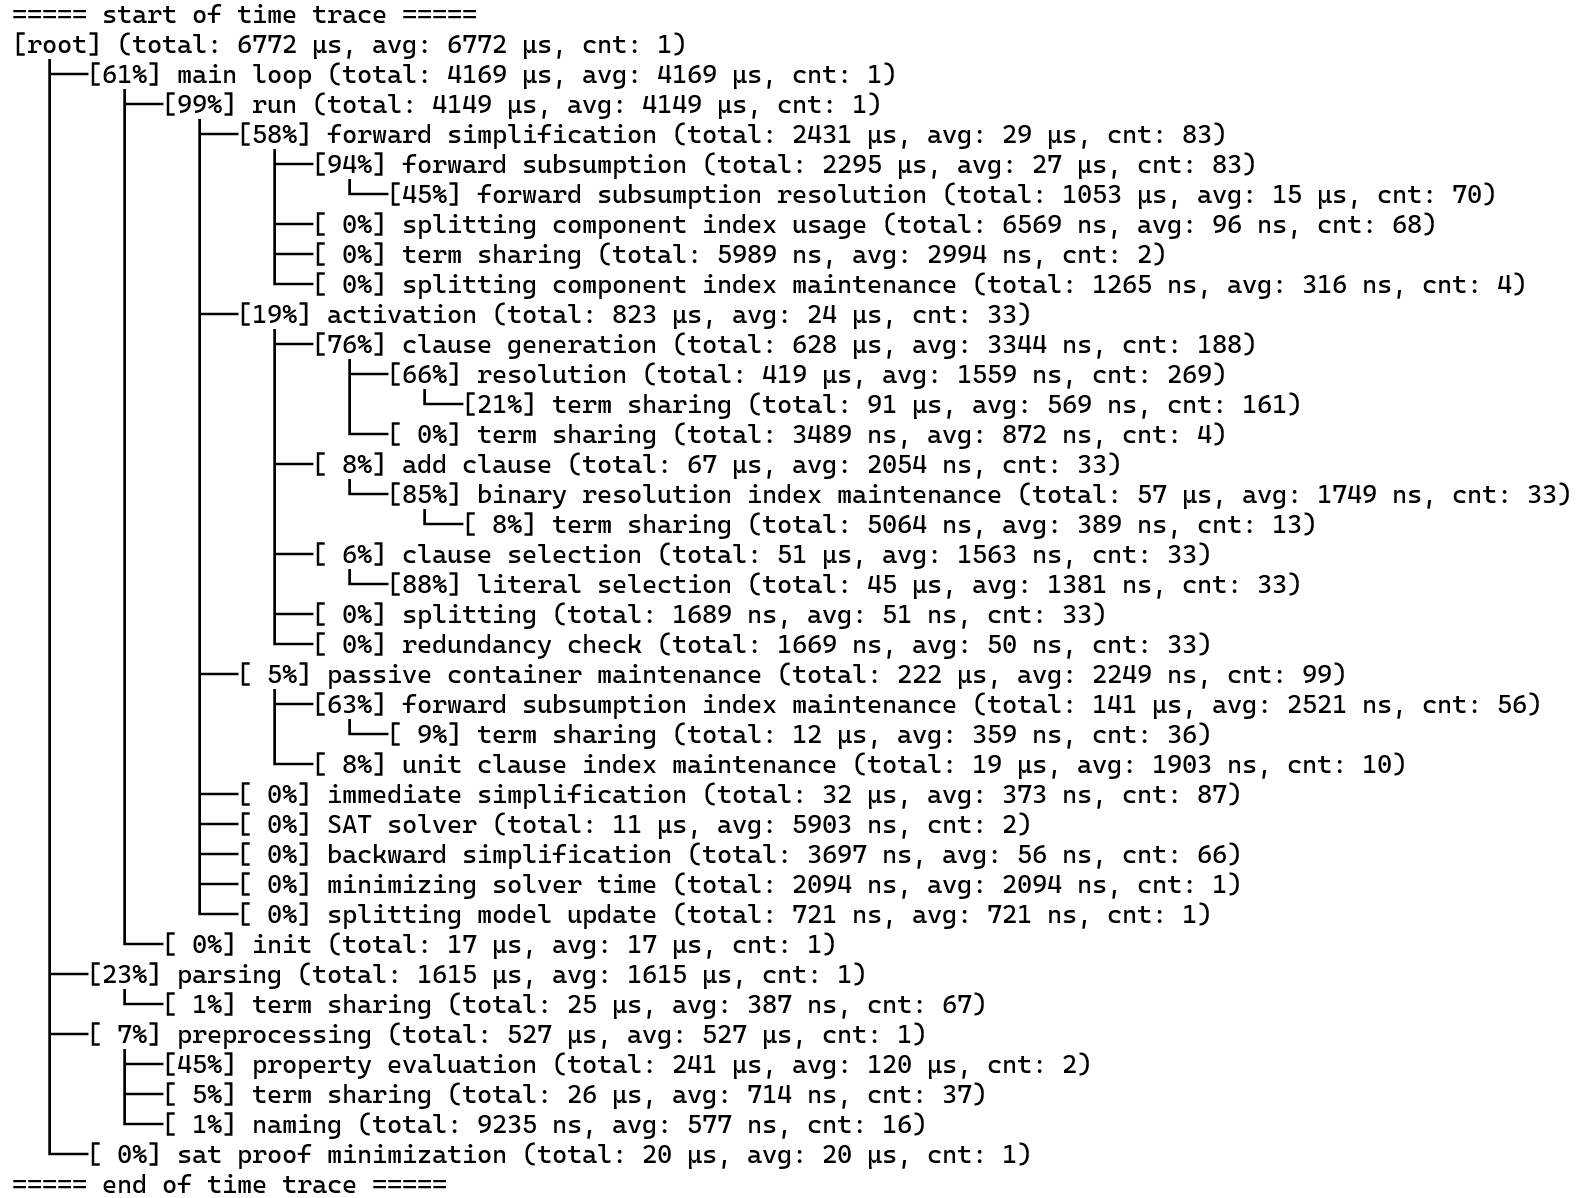
\includegraphics{images/3_vampire/time_profile.png}
    }
    \caption{Esempio di report di Time Trace}
    \label{fig:time_trace_report}
\end{figure}

Il terzo metodo non è serve a misurare il tempo di esecuzione ma conta il numero di invocazioni.
La macro \textit{RSTAT\_CTR\_INC(name)} definita in \textit{Debug/RuntimeStatistics} definisce 
un contatore associato ad ogni 'name' e lo incrementa di 1 ad ogni invocazione.
Anche in questo caso Vampire stamperà un report alla fine dell'esecuzione con il formato \textit{'name': 'count'}.
Vampire utilizza questa macro ad esempio per contare il numero di clausole create e il numero di clausole eliminate.
Un esempio di report è mostrato in figura \ref{fig:rstat_report}.

\begin{figure}[h]
    \centering
    \scalebox{0.5}{
        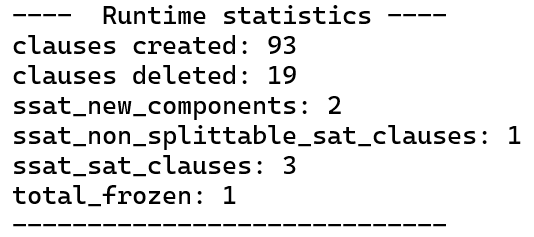
\includegraphics{images/3_vampire/runtime_statistics.png}
    }
    \caption{Esempio di report di Runtime Statistics}
    \label{fig:rstat_report}
\end{figure}


  
\end{document}